% 結果の章（数値は 図/values.tex と 図/tab_*.tex から。手で書かない）

% ============================================================
\chapter{主な検定}\label{ch:primary}

\begin{table}[H]
\centering\small
\caption{実現の TE と約束（3\%）の近さ（$g$ = 実現の TE ÷ 3\% の目安。1 なら約束どおり）}
\label{tab:tests}
\begin{adjustbox}{max width=\linewidth}
\begin{tabular}{@{}lrrrrrr@{}}
\toprule
比べたもの & $g$（前） & $g$（後） & 実現の TE（前 → 後） & $D$ & 95\% 区間 & 片側 $p$ \\
\midrule
\textbf{主：B と B＋校正}（2015 年末から、\V{primarydays} 日） & \V{primarygref} & \V{primarygnew} & \V{primaryteref} → \V{primarytenew} & \V{primaryD} & [\V{primarylo}, \V{primaryhi}] & \V{primaryp} \\
副：A と A＋校正 & \V{AvsAcalgref} & \V{AvsAcalgnew} & \V{AvsAcalteref} → \V{AvsAcaltenew} & \V{AvsAcalD} & [\V{AvsAcallo}, \V{AvsAcalhi}] & \V{AvsAcalp} \\
副：gpt-4o-mini、B と B＋校正（2023 年末から、\V{gptBvsBcaldays} 日） & \V{gptBvsBcalgref} & \V{gptBvsBcalgnew} & \V{gptBvsBcalteref} → \V{gptBvsBcaltenew} & \V{gptBvsBcalD} & [\V{gptBvsBcallo}, \V{gptBvsBcalhi}] & \V{gptBvsBcalp} \\
副：A＋校正と B＋校正 & \V{AcalvsBcalgref} & \V{AcalvsBcalgnew} & \V{AcalvsBcalteref} → \V{AcalvsBcaltenew} & \V{AcalvsBcalD} & [\V{AcalvsBcallo}, \V{AcalvsBcalhi}] & \V{AcalvsBcalp} \\
\bottomrule
\end{tabular}
\end{adjustbox}
\end{table}

評価する日は、2015 年末からの版では 2017 年以降、2023 年末からの版では 2024 年 7 月以降。実現の TE は $3\% \times g$。

\begin{keybox}[結果]
主な検定は\textbf{\V{primaryverdict}}された。株価で補正した共分散（B）に校正を足すと、2017 年以降の実現の TE は \V{primaryteref} から \V{primarytenew} になり、約束の 3\% にはっきり近づいた（片側 $p$ = \V{primaryp}）。
\end{keybox}

\begin{itemize}
\item \textbf{補正なしの共分散（A）でも}、校正で実現の TE は \V{AvsAcalteref} から \V{AvsAcaltenew} に近づいた。
\item \textbf{gpt-4o-mini の見通し}では、実現の TE が \V{gptBvsBcalteref} から \V{gptBvsBcaltenew} へと、大きく改善した。
\item \textbf{校正した後は、共分散の補正の差はなくなった}（A＋校正 \V{AcalvsBcalteref}、B＋校正 \V{AcalvsBcaltenew}、片側 $p$ = \V{AcalvsBcalp}）。
\end{itemize}

% ============================================================
\chapter{上限と実現の TE の動き}\label{ch:te}

\begin{figure}[H]
\centering
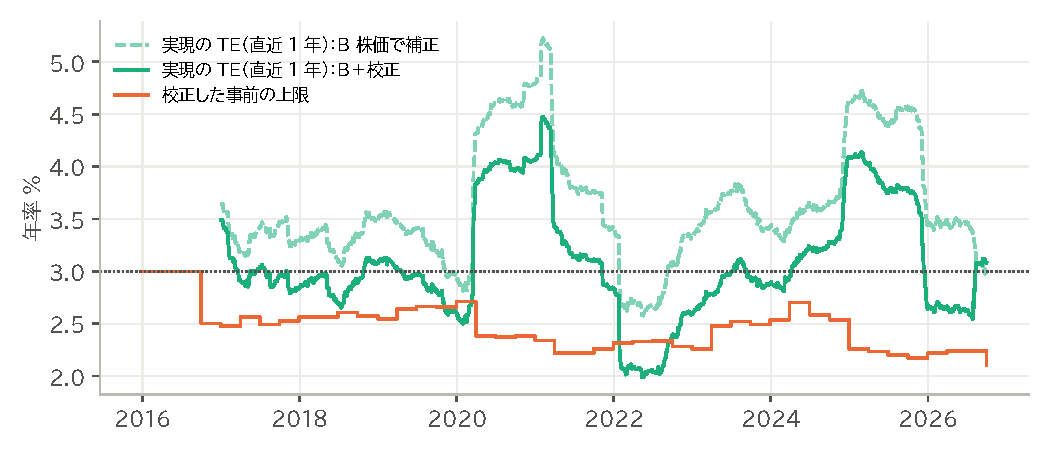
\includegraphics[width=\linewidth]{te.pdf}
\caption{2015 年末から四半期ごと、ChronoGPT＋リッジの見通し、共分散 B。直近 1 年の実現の TE（校正なしと校正あり）と、校正した事前の上限。点線は約束の 3\%。}
\label{fig:te}
\end{figure}

\begin{itemize}
\item 校正した上限は、多くの時期で年 2.1〜2.7\% だった（過去の偏りが 1.1〜1.4 程度で安定していた）。
\item それでも、2020 年の新型コロナの急落の後と、2025 年の前半には、実現の TE が 4\% を超えた。過去 3 年の偏りで割る規則は、変動が急に変わる時期には追いつかない（X03 と同じ）。
\item 落ち着いた時期（2018〜2019 年、2022〜2023 年）には、校正した版の実現の TE は 3\% の前後か、それより低かった。
\end{itemize}

% ============================================================
\chapter{すべての組み合わせ}\label{ch:runs}

\begin{table}[H]
\centering\small
\caption{2015 年 12 月末を 1 とした推移（2026 年 9 月末まで）。相手との差は年率。上限・実現の TE・$g$・情報レシオは評価する日（2017 年以降）のもの。情報レシオ = 比べる相手との差の年率 ÷ 実現の TE}
\label{tab:runs2015}
\tabin{runs_2015}
\end{table}

\begin{figure}[H]
\centering
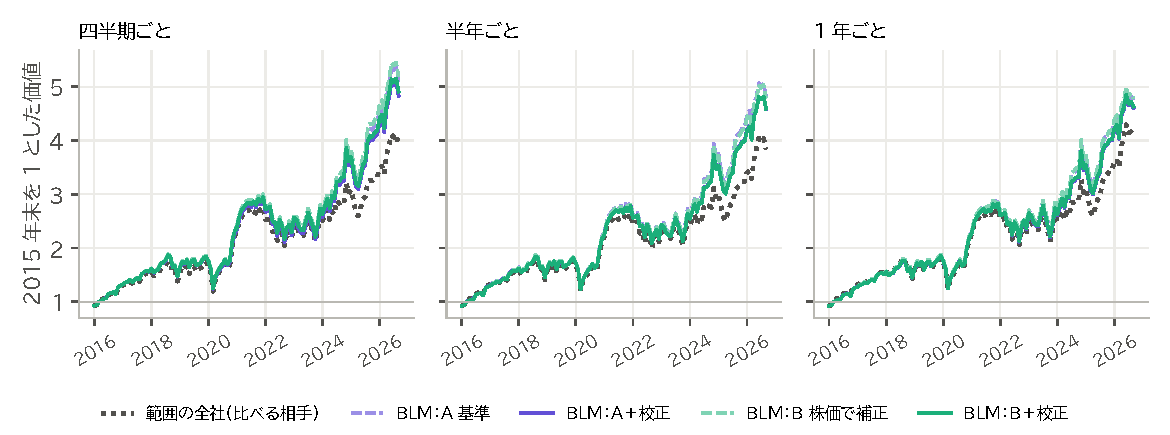
\includegraphics[width=\linewidth]{paths_2015_chrono_ridge.pdf}
\caption{2015 年末を 1 とした推移（ChronoGPT＋リッジの見通し）。}
\label{fig:paths2015}
\end{figure}

\begin{table}[H]
\centering\small
\caption{2023 年 12 月末を 1 とした推移（2026 年 9 月末まで）。上限・実現の TE・$g$・情報レシオは 2024 年 7 月以降}
\label{tab:runs2023}
\tabin{runs_2023}
\end{table}

\begin{figure}[H]
\centering
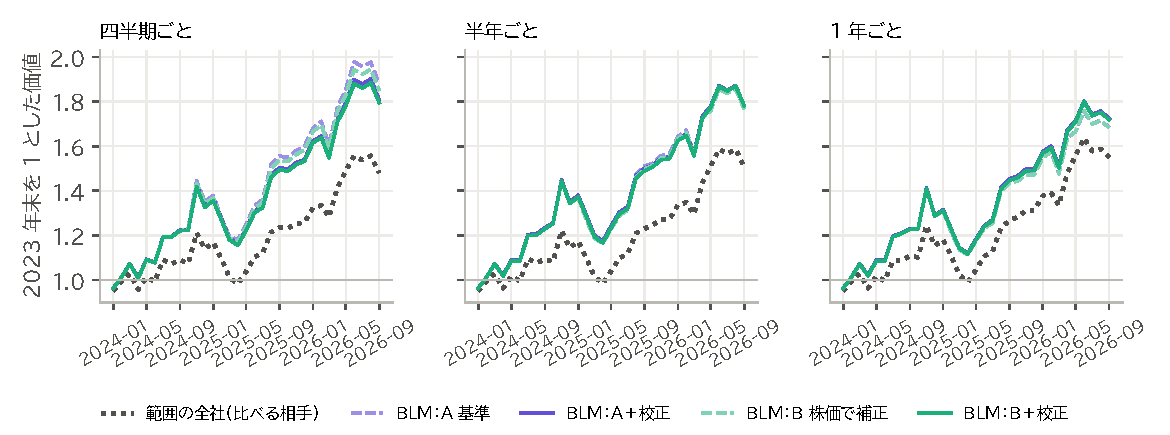
\includegraphics[width=\linewidth]{paths_2023_chrono_ridge.pdf}
\caption{2023 年末を 1 とした推移（ChronoGPT＋リッジの見通し）。}
\label{fig:paths2023c}
\end{figure}

\begin{figure}[H]
\centering
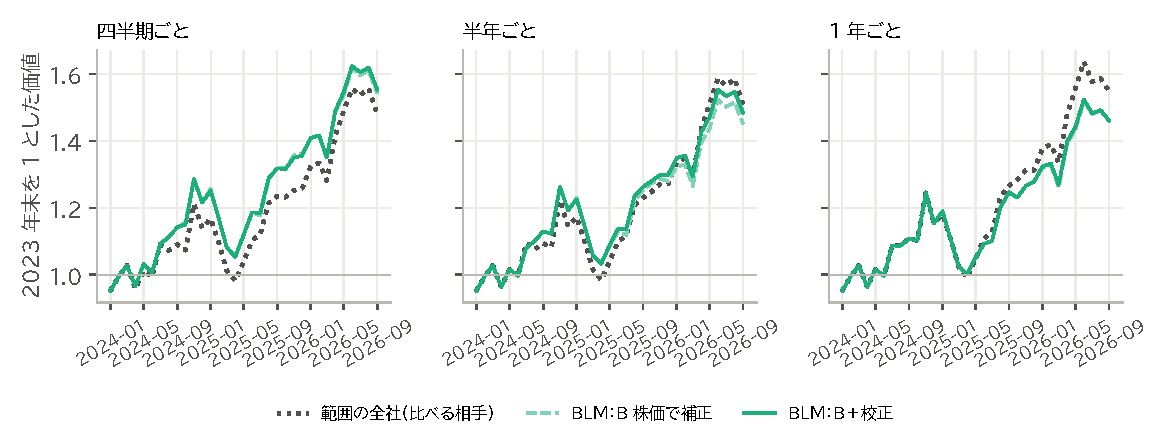
\includegraphics[width=\linewidth]{paths_2023_gpt_ridge.pdf}
\caption{2023 年末を 1 とした推移（gpt-4o-mini（重みを学習）の見通し）。}
\label{fig:paths2023g}
\end{figure}

\section{リスクとリターンの交換}

\begin{itemize}
\item 校正はリスクを小さくするので、比べる相手との差も小さくなる。2015 年末から四半期ごと（共分散 B）では、最終の値が \V{2015quarterchronoridgeBfinalvalue} から \V{2015quarterchronoridgeBcalfinalvalue}、相手との差が年 \V{2015quarterchronoridgeBannualexcessoverband} から \V{2015quarterchronoridgeBcalannualexcessoverband} になった。
\item リスク 1 単位あたり（情報レシオ）は、ほぼ変わらなかった（\V{2015quarterchronoridgeBireval} から \V{2015quarterchronoridgeBcalireval}。半年・1 年ごとでもほぼ同じか、わずかに良い）。
\item gpt-4o-mini の見通しでは、校正で情報レシオが良くなった（四半期ごとで \V{2023quartergptridgeBireval} から \V{2023quartergptridgeBcalireval}）。校正なしでは、事前の見積もりの 2 倍を超えるリスクを取っていた。
\end{itemize}

% ============================================================
\chapter{解釈}\label{ch:interpret}

\begin{enumerate}
\item \textbf{校正は効く}。過去 3 年の偏りで上限を割るだけで、実現の TE は約束の 3\% に近づいた。S\&P500 の X03 と同じ結果が、小型株の BLM でも、見通し（ChronoGPT・gpt-4o-mini）や共分散の作り方によらず得られた。
\item \textbf{校正した後は、共分散の補正（S3 の B）の差はなくなった}。S3 で B が偏りを小さくしたのは確かだが、その分は校正が吸収する。共分散の補正は、校正の前の「偏りの大きさ」を小さくするが、校正の後の「約束の守り方」は変えない。
\item \textbf{情報レシオは保たれた}。校正は、リスクとリターンを同じ割合で縮めるので、リスク 1 単位あたりの成績はほぼ変わらない。事前の見積もりが大きく外れていた gpt-4o-mini の見通しでは、むしろ良くなった。
\item \textbf{急な変化には追いつかない}。2020 年と 2025 年には、校正しても実現の TE が 4\% を超えた。過去の偏りを使う規則の限界である。
\end{enumerate}

\section{これからの BLM の標準}

\begin{itemize}
\item TE の上限に、この校正（過去 756 日の偏りで割る）を入れる。将来のデータを使わない規則なので、そのまま使える。
\item 報告書では「事前の TE の上限 3\%」でなく、「実現の TE はおよそ 3\%（評価する期間で \V{primarytenew}）」と書けるようになる。
\item 急な変化への対応（例えば VIX や直近 1 か月の変動率で上限を一時的に下げる、X04 の考え方）は、次の候補である。
\end{itemize}
